\documentclass[a4paper,11pt,oneside]{book}  %bylo report
\usepackage[margin=0.75in]{geometry}
\usepackage[utf8]{inputenc} %ISO-8859-2 
\usepackage[polish]{babel} 
%\usepackage{times} 
\usepackage[T1]{fontenc} 
\usepackage[MeX]{polski} 
\usepackage[pdftex]{graphicx} 
\usepackage{pdfpages} 
\usepackage{fancyhdr} %numery stron po zewnętrznej 
\usepackage{wrapfig}
\usepackage[colorlinks=true,bookmarksopen,plainpages=false,urlcolor=blue,citecolor=black,filecolor=black,linkcolor=black,,unicode]{hyperref} 
\usepackage{titlesec} 
\usepackage{booktabs}
\usepackage{attachfile}
\usepackage{appendix}
\usepackage{listings}
\usepackage{tikz}
\usetikzlibrary{shapes,arrows,fit} %use shapes library if you need ellipse
\title{Sprawozdanie z projektu SPEKTROP\\ Blok elektroniki spektrometru obrazującego \\[10pt] \large{Creotech Instruments S.A.} \\ \large{Centrum Badań Kosmicznych}}
%\author{Piotr Zdunek}

\usepackage{newunicodechar}
\newunicodechar{fi}{fi}
\usepackage{courier}
\usepackage{listings}
\usepackage{float}
\pdfminorversion=5 
\pdfcompresslevel=9
\pdfobjcompresslevel=2
\usepackage{multirow}
\usepackage{url}
\usepackage{graphics}
\usepackage[section]{placeins}
\usepackage{hyperref}


\begin{document}
%\maketitle 
%
%\begin{table}[h]
%  \centering
%  \begin{tabular}{| c | c | c |}
%    \cline{1-3}  \textbf{Skład zespołu} & \textbf{Przedmiot} & \textbf{Data} \\
%   \hline
% 	Piotr Zdunek 	& \multirow{2}{*}{ Metody i~systemy pomiarowe wielkiej częstotliwości} & \multirow{2}{*}{07.04.2014} \\[5pt]
% 	Paweł Gontarek & & \\
%   \hline
%   \textbf{Prowadzący} 		& \textbf{Tytuł ćwiczenia}	&	\textbf{Numer stanowiska} \\
%   \hline
%   dr~inż. Wojciech Wiatr	&	Pomiar parametrów materiałowych metodą rezonansową	&	2			\\
%   \hline
%  \end{tabular}
%    \label{tab:tytulowa}
%\end{table}





\maketitle


\lstdefinestyle{custom}{
  belowcaptionskip=1\baselineskip,
  breaklines=true,
  frame=L,
  xleftmargin=\parindent,
  language=Matlab,
  showstringspaces=false,
  basicstyle=\footnotesize\ttfamily,
  keywordstyle=\bfseries\color{green!40!black},
  commentstyle=\itshape\color{purple!40!black},
  identifierstyle=\color{blue},
  stringstyle=\color{orange},
}

\lstset{escapechar=@,style=custom}

%\tableofcontents
%\newpage	
\chapter{Wstęp} 
Poniższy dokument jest sprawozdaniem z projektu bloku elektroniki spektrometru obrazującego SPEKTROP zaprojektowanego przez Creotech Instruments S.A. na zlecenie Centrum Badań Kosmicznych. Zawarto w nim specyfikację systemu, sposób działania oraz opis zastosowanych rozwiązań sprzętowych i programowych. 

Projekt SPEKTROP jest systemem kamery spektralnej, umieszczonej na samolocie bądź UAV\footnote{UAV - Unmanned Aerial Vehicle} pozwalającym na rejestrację obrazu lądu jednocześnie w wielu długościach fali.
Takie rozwiązanie pozwala na analizę powierzchni różnych rodzajów obszarów jak lasy, jeziora, pola uprawne. Czy analizę możliwości wystąpienia złóż.

\begin{figure}[htp]
	\centering
	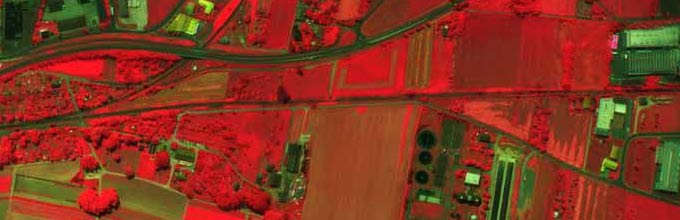
\includegraphics[width=12cm]{spektrop_ex.jpg}
	\caption{Przykładowy obraz z kamery spektralnej\cite{SPEC_PHOTO}}
	\label{fig:EX_PHOTO}
\end{figure}


Sercem zaprojektowanego urządzenia jest układ SoC Zynq Z7045, który łączy w sobie układ FPGA Kintex 7 oraz dwurdzeniowy procesor ARM Cortex-A9. System pozwala na rejestrację danych z czujnika CMV4000 z maksymalną prędkością 100 FPS przy minimalnym czasie ekspozycji wynoszącym $\sim$ 10 ms.Ponadto system umożliwia rejestrację parametrów lotu niezależnie od akwizycji obrazu oraz z możliwością przyporządkowania danych do poszczególnych klatek. Dzięki czemu możliwa jest późniejsz analiza zebranych danych. Zebrane dane są zapisywane na dysku/ach HDD poprzez interfejs SATA zaimplementowanym w logice FPGA przy pomocy transceiverów GTX.

Sterowanie i komunikacja z systemem odbywa się poprzez interfejs Ethernet przy pomocy dedykowanej aplikacji działającej pod systemem Linux. 


\chapter{Specyfikacja}

\section{Czujnik CMOS}
\begin{itemize}
	\item Detektor: CMV4000 \cite{CMV4000} albo CIS 1910F \cite{CIS}.
	\item Tryby pracy czujnika:
		\begin{itemize}
			\item Podstawowy: czas ekspozycji (EXP\footnote{EXP - Exposure}) 1-10 ms, 100 FPS\footnote{FPS -Frames Per Second}
			\item Manualny:	dowolnie długi czas ekspozycji z mniejszą ilością FPS (np. 5-10 FPS przy EXP $\sim$ 1-2 ms
		\end{itemize}

	\item Rozdzielczość bitowa - 16 bit/piksel, ENOB\footnote{ENOB - Effective Number of Bits}:8-9 bitów
	\item Zakres temperatury pracy: $-10^{o}C \div +50^{o}C$

\end{itemize}

\section{Platforma sprzętowa}
\begin{itemize}
\item Xilinx Zynq Evaluation Board ZC706 \cite{ZC706}
\end{itemize}

\section{System rejestracji parametrów lotu}

\begin{itemize}
\item rejestracja parametrów lotu na podstawie systemów GPS oraz IMU\footnote{IMU - Internal Management Unit} z zapewnieniem synchronizacji czasowej względem akwizycji klatek i niezależnie 
	\begin{itemize}
	\item minimalny okres zapisu parametrów - 0.1 s
	\end{itemize}
\item zapis czasu pomiaru (timestamp) i czasu akwizycji parametrów lotu
\item nośnikiem danych jest dysk twardy 
%(SSD\footnote{SSD - Solid State Drive}/HDD\footnote{HDD - Hard Disk Drive}) z interfejsem SATA,
(SSD/HDD) z interfejsem SATA, zapis odbywa się przy pomocy interfejsu GTX
\end{itemize}



\section{Tryby pracy}

\begin{itemize}
\item Ręczny - ustawiany przez operatora przy pomocy komputera PC (operator leci w samolocie)
\item Autonomiczny - posiadający następujące funkcje: 
	\begin{itemize}
		\item wyliczanie ekspozycji i częstotliwości akwizycji klatek na podstawie parametrów lotu dostarczanych przez systemy sterujące samolotu/UAV
		\item sprawdzanie poprawności ekspozycji
		\item możliwość wyzwalania pomiarów na podstawie osiągnięcia pozycji wskazanej przez GPS
	\end{itemize}
	
\end{itemize}

\section{Wymagania elektryczne}

Napięcie zasilania 24 V albo 12 V. 

\section{Wymagania mechaniczne}

Wymiary PCB: 85 mm x 160 mm. 


\section{Proponowany schemat funkcjonalny systemu}

\begin{figure}[!h]
	\centering
	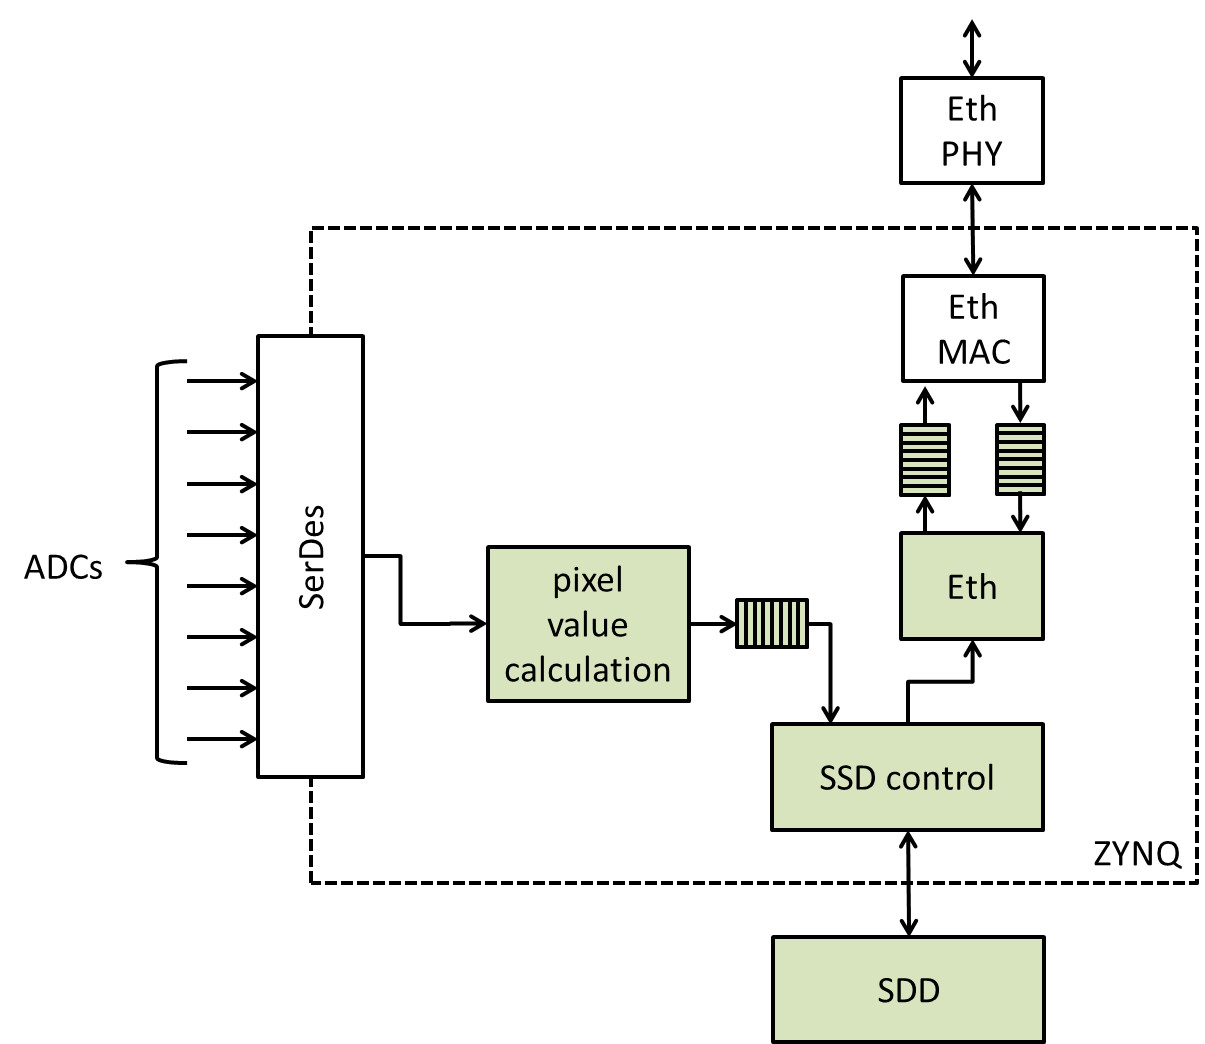
\includegraphics[width=12cm]{schemat_cbk.jpg}
	\caption{Schemat blokowy systemu}
	\label{fig:SYS}
\end{figure}


%\section{Założenia}

\chapter{Koncepcja realizacji}

Poniższy rozdział opisuje koncepcję realizacji bloku elektroniki projektu SPEKTROP. Rysunek [\ref{fig:OVER}] przedstawia główne elementy systemu: 
\begin{itemize}
	\item płytę ewaluacyjną ZC706
	\item czujnik CMOSIS MV4000
	\item interfejs SATA
	\item interfejs Ethernet
	\item połączenie z systemem GPS i IMU
\end{itemize}
\begin{figure}[!h]
	\centering
	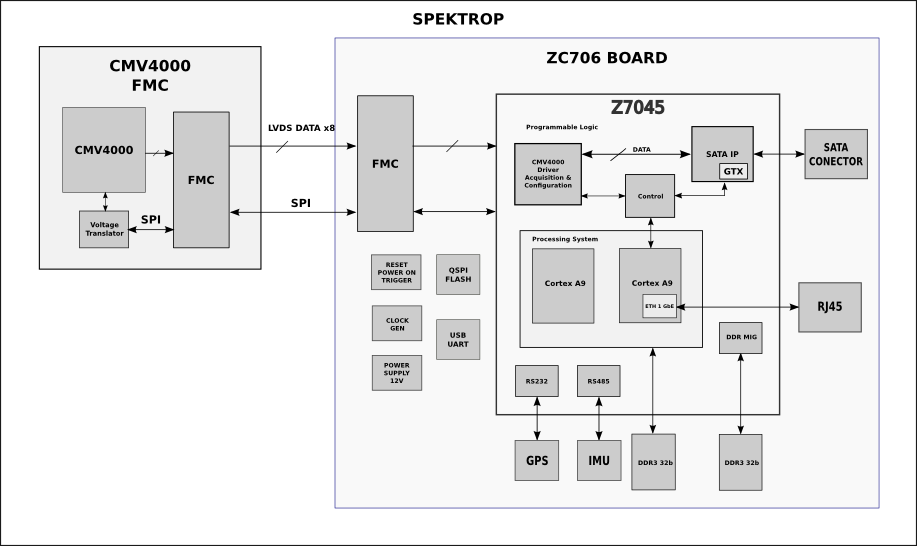
\includegraphics[width=16cm]{systembnw2.png}
	\caption{Główne elementy systemu}
	\label{fig:OVER}
\end{figure}

Całość funkcjonalności systemu jest realizowana za pomocą układu SoC Zynq. Akwizycja danych i zapis na dysku poprzez interfejs SATA zostanie zrealizowany w logice programowalnej, natomiast kontrola i zarządzanie w dwurdzeniowym procesorze ARM Cortex A9. 

Logika programowalna pozwala na przesył i prostą analizę dużej ilości danych. Czujnik CMV4000 wysyła dane do układu Zynq szeregowo 8 liniami LVDS, dane w FPGA są deserializowane i przesyłane poprzez wewnętrzne magistrale do IP SATA. Zapis na dysku jest realizowany przy pomocy transceiverów GTX.


Zarządzanie jest realizowane głównie za pomocą jednego rdzenia ARM, na którym uruchomiony jest system czasu rzeczywistego FreeRTOS wraz z obsługą stosu TCP/IP. Drugi rdzeń odpowiada za obsługę przerwania IP AXI VIDEO DMA.

Po akwizycji każdej klatki, zapisywane są parametry lotu związane z daną klatka oraz dotyczące samej akwizycji. Niezależnie od tego na karcie pamięci zapisywane są dane z parametrów lotu oraz dane diagnostyczne systemu. 


\chapter{Realizacja}
Niniejszy rozdział zawiera opis techniczny realizacji bloku elektroniki do projektu SPEKTROP. W pierwszej części opisano wykorzystany układ SoC Zynq oraz czujnik CMV4000. Następnie przedstawiona została 

Rysunek [\ref{fig:OVER}] zawiera schemat blokowy systemu. System składa się z modułu ewaluacyjnego układu Zynq ZC706, oraz z modułu FMC z czujnikiem CMOSIS CMV4000.
%\subsection{Wstęp}

\begin{figure}[!h]
	\centering
	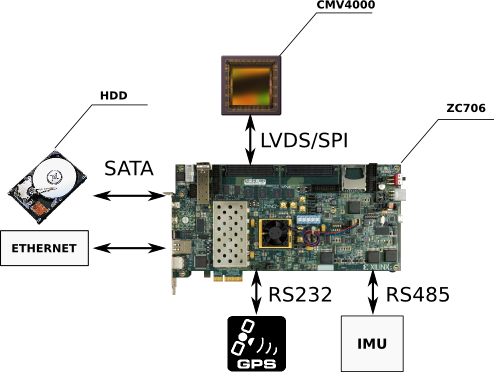
\includegraphics[width=12cm]{OVER2.png}
	\caption{Główne elementy systemu}
	\label{fig:OVER}
\end{figure}

\section{Platforma sprzętowa}
System oparty jest o moduł ewaluacyjny ZC706 posiadający wszystkie podstawowe komponenty sprzętowe potrzebne do realizacji zaawansowanych systemów przetwarzania.

\begin{figure}[H]
	\centering
	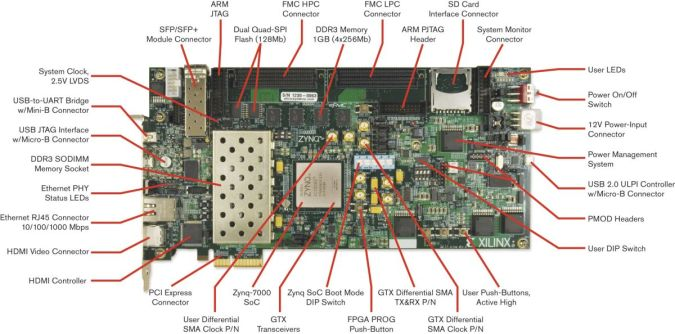
\includegraphics[width=12cm]{zc706-base-board.jpg}
	\caption{Elementy płyty ewaluacyjnej ZC706}
	\label{fig:ZC706}
\end{figure}

Moduł posiada następujące komponenty:
\begin{itemize}
\item Układ SoC
	\begin{itemize}
	\item Zynq-7000 XC7Z045 FFG900 
	\end{itemize}
	
\item Konfiguracja
	\begin{itemize}
	\item 2X16MB Quad SPI Flash
	\item SDIO 
	\item PC4 i JTAG 
	\end{itemize}

\item Pamięć
	\begin{itemize}
	\item DDR3 Component Memory 1GB (PS)
	\item DDR3 SODIM Memory 1GB (PL)
	\item 2X16MB Quad SPI Flash
	\item IIC - 1 KB EEPROM
	\end{itemize}
	
\item Interfejsy komunikacyjne
	\begin{itemize}
	\item PCIe Gen2x4
	\item SFP+ and SMA Pairs
	\item GigE RGMII Ethernet (PS)
	\item 1 CAN with Wake on CAN (PS)
	\item USB OTG 1 (PS) - Host USB
	\item IIC Bus Headers/HUB (PS)
	\item USB UART (PS)
	\end{itemize}

\item Komponenty wideo
	\begin{itemize}
	\item HDMI 8 color RGB 4.4.4 1080P-60 OUT
	\item HDMI IN 8 color RGB 4.4.4
	\end{itemize}
	
\item Złącza we/wy
	\begin{itemize}
	\item FMC LPC 
	\item FMC HPC
	\item Pmod dualny i pojedynczy
	\item Dostęp do I2C
	\item USB OTG 1 (PS) - Host USB
	\item IIC Bus Headers/HUB (PS)
	\item USB UART (PS)
	\end{itemize}
	
\item Sygnały zegarowe
	\begin{itemize}
	\item 33MHz Zegar systemowy
	\item 200MHz PL Oscylator
	\item złącza SMA dla zewnętrznych sygnałów zegarowych
	\item referencyjne do GTX 
	\item OBSAI/CPRI – SFP+ 
	\item EXT Config CLK
	\end{itemize}

\item Sterowanie
	\begin{itemize}
	\item 2 User Push Buttons/Dip Switch, 2 User LEDs
	\item 3 User Push Buttons, 2 User Switches, 8 User LEDs
	\item IIC access to 8 I/O
	\item IIC access to a WTClock
	\end{itemize}

\item Zasilanie
	\begin{itemize}
	\item 12 V 
	\item możliwość pomiaru prądu linii zasilających
	\end{itemize}
\end{itemize}

\section{Układ SOC Zynq}
Układy z serii Zynq 7000 stanowią najnowszą generację układów typu SOC FPGA – stanowią połączenie na jednym kawałku krzemu programowalnych układów logicznych FPGA serii 7 z dwurdzeniową procesorem ARM Cortex A9 oraz szeroką paletą peryferiów takich jak Ethernet, SPI, I2C, CAN, USB, itp. Połączenie takie upraszcza tworzenie oraz obniża koszty złożonych systemów wbudowanych. Układ Zynq 7020 używany w projekcie posiada 32 bitowy interfejs do pamięci DDR3 współdzielony pomiędzy procesorem, a logiką programowalną. Zapewnia to bardzo dużą przepustowość danych pomiędzy procesorem a FPGA. Od strony logiki programowalnej dostęp do pamięci realizowany jest przez 4 złącza AXI HP (wysokiej przepustowości). Maksymalna, teoretyczna przepustowość pojedynczego kanału HP wynosi 1200MB/s w każdą stronę. Maksymalna, teoretyczna, całkowita przepustowość pamięci DDR3 w układzie wynosi 4264 MB/s. Dodatkowo układ posiada po dwa złącza AXI GP (ogólnego przeznaczenia) master i slave między procesorem a układem FPGA o przepustowości 600MB/s w każdą stronę. Najczęściej wykorzystywane są one do programowania rejestrów peryferiów zrealizowanych w logice programowalnej. Układ Zynq w wersji 7020 ma 85 tysięcy programowalnych komórek logicznych, 106400 przerzutników, 220 układów DSP oraz 560KB BRAM. Rdzenie ARM Cortex pracują z zegarem 667MHz.
\subsection{Architektura APU}
Każdy z rdzeni posiada po 32KB pamięci podręcznej instrukcji oraz danych, układ MMU, FPU oraz NEON SIMD. Rdzenie dzielą między sobą pamięć podręczną drugiego poziomu o rozmiarze 512 KB, kontroler przerwań UART, OCM oraz pamięć DDR.
\section{Sensor CMV4000}
Sensor użyty w projekcie to przetwornik video o rozmiarze 1”, wykonany w technologii CMOS. Charakteryzuje się rozdzielczością 2048x2048 punktów i maksymalną szybkością przetwarzania ramek obrazu o wartości 180 klatek/s przy zegarze o częstotliwości 480 MHz (maksymalna częstotliwość zegara dla tego sensora). Sensor posiada 2 wejścia zegarowe – zegar systemowy oraz zegar LVDS. Programowanie rejestrów sensora odbywa się przy pomocy interfejsu SPI. Dane z przetwornika wystawiane są na 16 (lub mniej w zależności od ustawień) wyjść LVDS. Dodatkowo sensor posiada jeszcze 1 wyjście sterujące LVDS, na które wystawiane są sygnały sterujące strumieniem danych oraz 1 wyjście zegara LVDS danych. Dane wystawiane są z częstotliwością równą połowie częstotliwości zegara podanego na wejście zegarowe LVDS na obu zboczach zegara (DDR). Dane na poszczególnych liniach LVDS są wysyłane przez sensor w postaci szeregowej – ze współczynnikiem 10:1 lub 12:1 (w zależności od ustawień przetwornika AC). Wysyłanych jest równolegle 16 serializowanych fragmentów ramki obrazu – po jednym na każde wyjście LVDS. Aby odtworzyć pierwotną postać obrazu, należy najpierw zdeserializować, a następnie przegrupować dane otrzymane od sensora.

\begin{figure}[H]
	\centering
	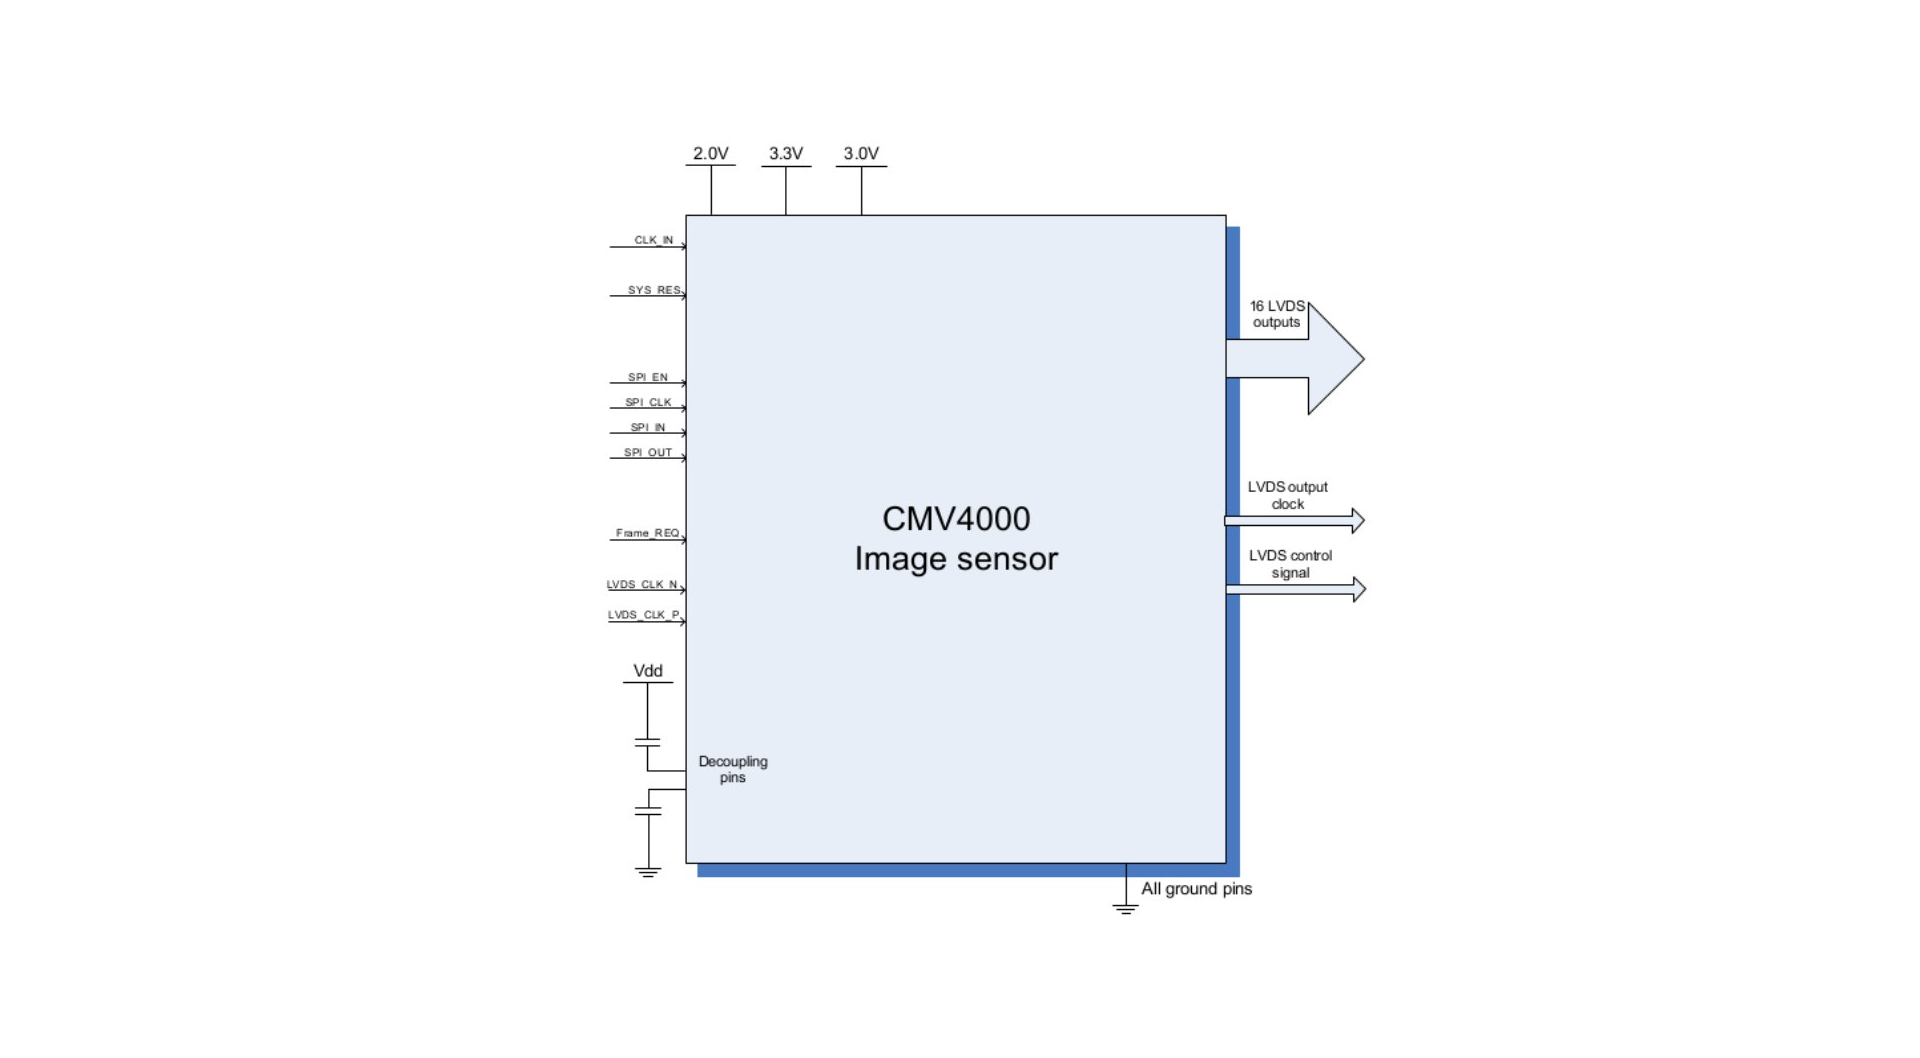
\includegraphics[width=18cm]{cmv4000.png}
	\caption{Schemat połączeń sensora CMV4000}
	\label{fig:CMV4000}
\end{figure}

\section{Część sprzętowa (logika programowalna)}
Część sprzętowa projektu składa się z pliku konfiguracyjnego układu SOC FPGA wygenerowanego na podstawie list połączeń utworzonych przez kreatory IP – core oraz na podstawie kodu VHDL. Zadaniem modułu sprzętowego jest wysyłanie sygnałów sterujących do sensora oraz odbieranie danych z sensora, odpowiednie ich przetwarzanie i zapisywanie w pamięci RAM systemu. Dalszym przetwarzaniem zajmuje się część programowa projektu, działająca na dwóch rdzeniach procesora ARM Cortex A9.

\begin{figure}[H]
	\centering
	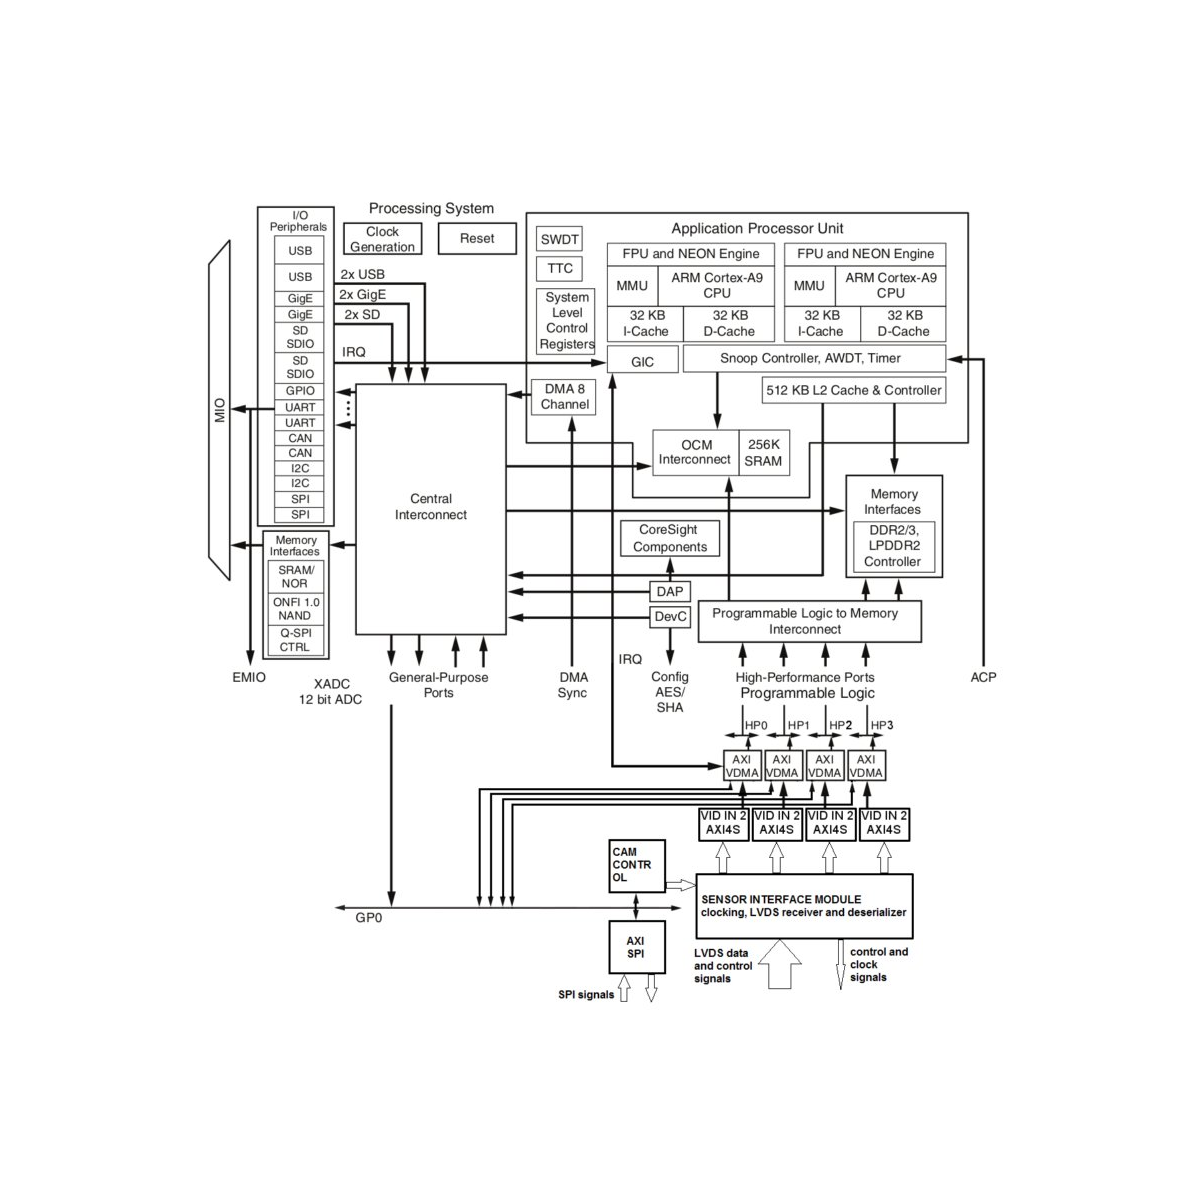
\includegraphics[width=16cm]{fpga.png}
	\caption{Schemat konfiguracji sprzętowej układu Zynq}
	\label{fig:Zynq}
\end{figure}

W części sprzętowej wykorzystano zarówno gotowe rdzenie IP dostarczane nieodpłatnie przez firmę Xilinx jak i własny kod VHDL. Jak widać na rysunku 2, układ został skonfigurowany w taki sposób, aby wykorzystać wszystkie dostępne łącza wysokiej przepustowości (HP0 - HP3) pomiędzy logiką programowalną, a kontrolerem pamięci DDR RAM. Pozwala to na optymalne dopasowanie się do szerokości szyny kontrolera pamięci, która wynosi 64 bity. Zdeserializowane dane z sensora po uzupełnieniu zerami mają szerokość równą 4x64bity. Wykorzystano także jeden port ogólnego przeznaczenia (GP0), do komunikacji z rdzeniami IP. Maksymalna przepustowość danych pomiędzy sensorem, a interfejsem FPGA wynosi: 180kl./s*2048*2048*10bit = 7200Mbit/s. Przepustowość ta jest sztucznie zwiększana na ścieżce pomiędzy modułem interfejsu LVDS, a rdzeniami AXI VIDEO DMA, ponieważ linie danych na magistralach AXI muszą mieść szerokość równą wielokrotności 8 bitów. Rozmiar próbki jest więc uzupełniany zerami do szerokości 16 bitów w module interfejsu LVDS i w takiej postaci przesyłany do rdzeni VID IN 2 AXI4S. Zwiększa to wykorzystywaną część przepustowości do maksymalnie 11520Mbit/s = 1440MB/s. W projekcie ta wartość jest nieco mniejsza, ponieważ sensor nie jest taktowany z maksymalną częstotliwością.

\subsection{Przepływ danych w FPGA}
\begin{figure}[H]
	\centering
	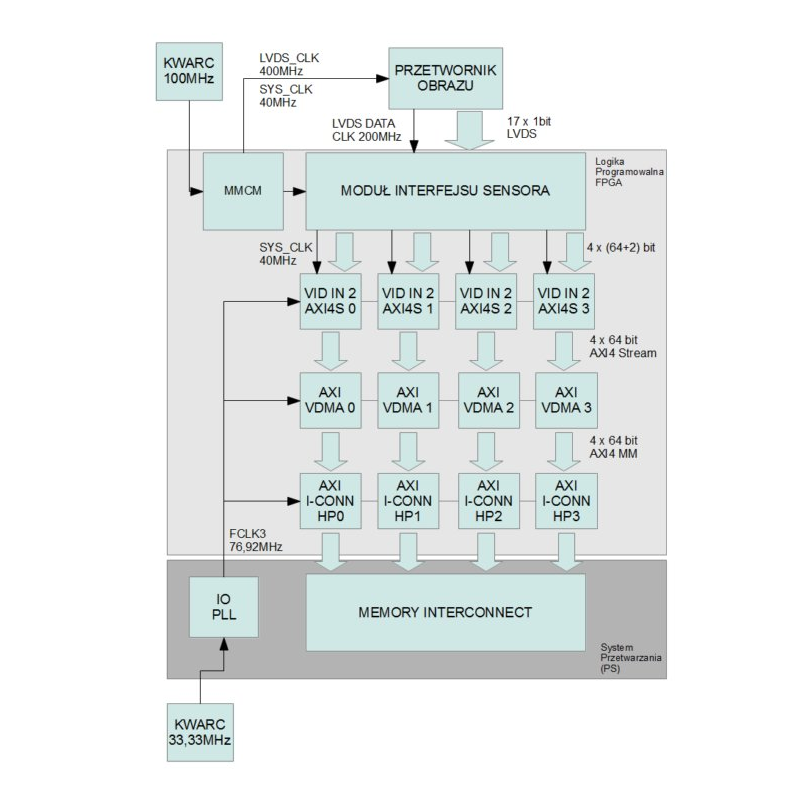
\includegraphics[width=14cm]{data.png}
	\caption{Przepływ danych z czujnika do logiki}
	\label{fig:Zynq2}
\end{figure}
 
 Rysunek [\ref{fig:Zynq2}] przedstawia schemat modułów sprzętowych przetwarzających i przesyłających dane obrazowe z sensora. Na rysunku pominięto interfejs SPI oraz interfejsy AXI4 Lite. W projekcie wykorzystano 2 układy PLL do generacji zegarów dla systemu – jeden zasilany z kwarcu procesora i generujący zegar 76,92 MHz dla rdzeni IP oraz drugi zasilany z kwarcu przeznaczonego dla FPGA i generujący zegary o różnych częstotliwościach (wyszczególnionych poniżej) dla Modułu interfejsu sensora.
 
\begin{figure}[H]
	\centering
	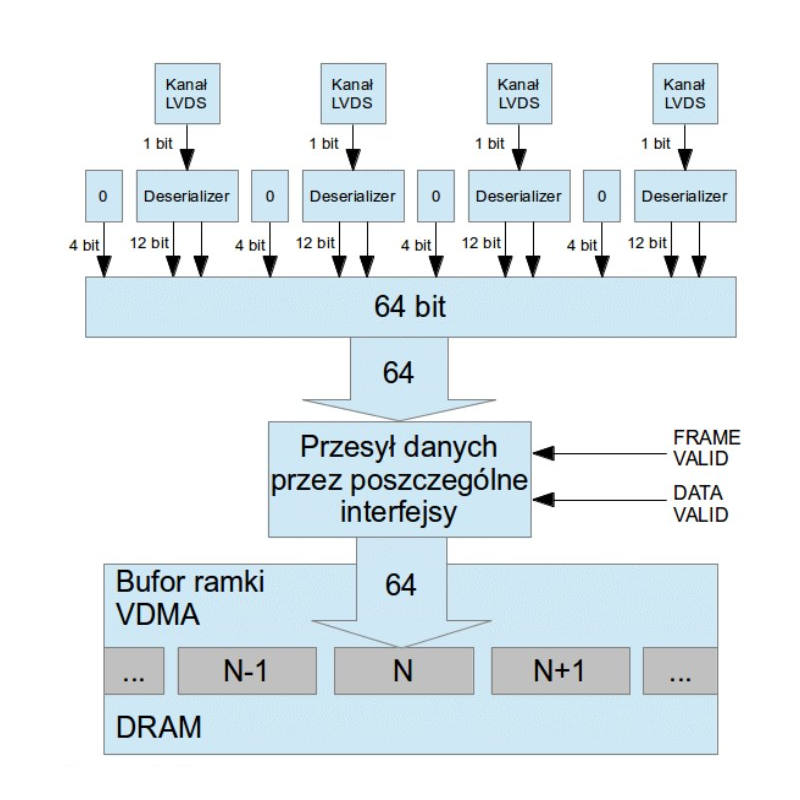
\includegraphics[width=14cm]{data2.png}
	\caption{Deserializacja i buforowanie danych}
	\label{fig:Zynq3}
\end{figure}

Na rysunku 4 przedstawiono uszczegółowienie jednej z 4 ścieżek przepływu danych obrazu w systemie. Na każdą ścieżkę przypadają 4 z 16 kanałów danych LVDS. 1 kanał sterujący LVDS jest współdzielony pomiędzy ścieżkami (dane sterujące są takie same dla wszystkich kanałów danych). Jak wynika z przedstawionego rysunku oraz sposobu przesyłania danych przez sensor [1], dane w pamięci nie są układane w kolejności odpowiadającej ich położeniu w obrazie i muszą zostać uporządkowane przed generowaniem podglądu lub zapisu do formatu obrazowego. Porządkowanie danych odbywa się programowo.

\subsection{Wykorzystywane interfejsy komunikacyjne}
\begin{itemize}
\item AXI4 – Stream 
\item AXI4 – Lite 
\item AXI4 – Memory Mapped
\end{itemize}


\subsection{Domeny zegarowe} 

W projekcie wykorzystywane są następujące domeny zegarowe:
\begin{itemize}
\item FCLK\_CLK3 – 76,92308 MHz, zegar systemowy, generowany w PLL układu Zynq
\item SYS\_CLK – 40MHz, główny zegar modułu interfejsu sensora, główny zegar sensora oraz zegar pikseli po deserializacji, generowany w PLL układu Zynq
\item SPI\_CLK – FCLK\_CLK3/32, zegar SPI generowany w rdzeniu AXI SPI z głównego zegara systemowego
\item ZEGAR DANYCH LVDS – 200MHz, zegar odbiorczy danych LVDS, generowany w PLL układu Zynq
\item ZEGAR LVDS SENSORA – 400MHz, zegar nadajnika LVDS sensora, generowany w PLL układu Zynq
\end{itemize}

Sensor CMV4000 generuje dodatkowo własny sygnał zegarowy danych LVDS, o częstotliwości równej połowie częstotliwości wejściowego zegara LVDS, ale nie jest on wykorzystywany w projekcie.

\subsection{Opis modułów IP}
\subsubsection{AXI Video Direct Memory Access 5.04.a}
AXI VDMA jest modułem własności intelektualnej dostarczanym nieodpłatnie przez firmę Xilinx wraz z licencją na oprogramowanie projektowe ISE Design Suite do układów SOC oraz FPGA tej firmy. Moduł ten oferuje dwukierunkowe łącze wysokiej przepustowości pomiędzy peryferiami o interfejsie zgodnym z protokołem AXI4 – Stream Video, a pamięcią (w tym przypadku pamięcią DDR RAM). Zarządzanie modułem odbywa się poprzez zapisywanie oraz odczytywanie zestawu rejestrów poprzez interfejs AXI4 – Lite. Moduł obsługuje interfejs AXI4 Memory Map o szerokościach 32, 64, 128, 256, 512 oraz 1024 bitów oraz interfejs AXI4 – Stream o szerokościach do 1024 bitów, przy czym szerokość ta musi być wielokrotnością 8. Rzeczywista szerokość szyny do pamięci wynosi 64 bity, w związku z czym większe szerokości są dzielone na 64 bitowe transfery. AXI VDMA ma możliwość przechowywania w pamięci zewnętrznej do 32 ramek obrazu. Moduł zapewnia podstawową możliwość obsługi błędów – błędne wartości podstawowych parametrów pracy są wykrywane, a informacja o nich jest zapisywana na poszczególnych bitach odpowiednich rejestrów. AXI VDMA może generować przerwanie na zaprogramowanym przez użytkownika zdarzeniu takim jak wystąpienie błędu, odliczenie zadanej ilości klatek lub odliczenie zadanego opóźnienia względem początku klatki.

\begin{figure}[H]
	\centering
	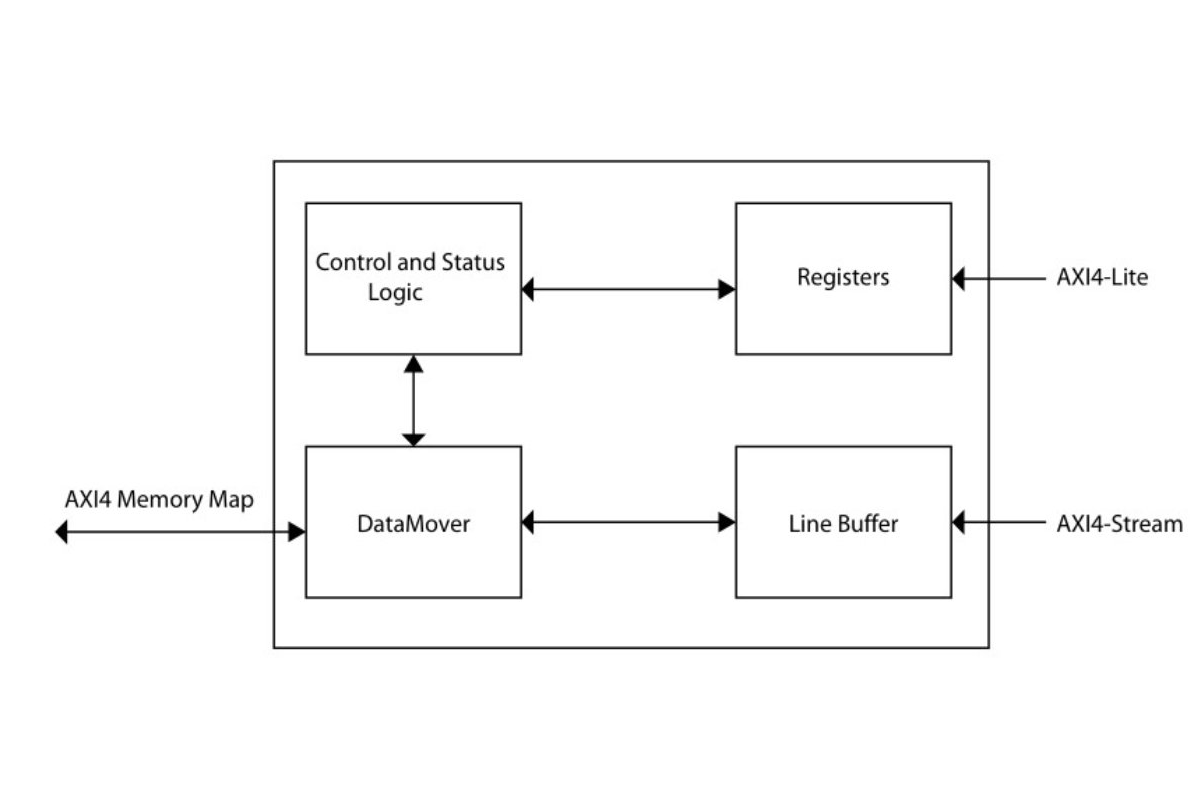
\includegraphics[width=14cm]{data3.png}
	\caption{Przepływ danych w magistralach AXI}
	\label{fig:Zynq3}
\end{figure}

\subsubsection{Video In to AXI4 – Stream 2.01.a} 

Podobnie jak AXI VDMA moduł ten jest udostępniany nieodpłatnie przez firmę Xilinx. Jego zadaniem jest dostarczanie interfejsu pomiędzy źródłami cyfrowego, równoległego sygnału wideo (np. z przetworników wideo, interfejsu HDMI, DVI itp.), a magistralą protokołu AXI4 – Stream Video. Moduł zapewnia przejście pomiędzy dwoma domenami zegarowymi – zegarem pikseli sygnału wideo oraz zegarem magistrali AXI4 Stream. Obsługiwana jest większość formatów cyfrowego wideo, z długościami próbek na kanał do 16 bitów. Moduł posiada także wejściową kolejkę FIFO, która pozwala na zastosowanie zegara AXI, o częstotliwości mniejszej od zegara pikseli. Jest to możliwe, ponieważ protokół AXI4 Stream przesyła tylko aktywne piksele obrazu. 

Minimalnym zestawem sygnałów sterujących wideo potrzebnych do poprawnego działania modułu jest para DE, Vsync. Sygnały te są niezbędne do ustalenia granic końca linii oraz początku nowej ramki. W projekcie do wejścia DE został podłączony sygnał Data Valid sensora, a do wejścia Vsync sygnał Frame Valid, uprzednio zdeserializowane z kanału sterującego LVDS. W projekcie nie jest wykorzystywany moduł Video Timing Controller. 

Sensor CMV4000 wystawia sygnały Frame Valid oraz Data Valid na tym samym zboczu zegara, natomiast jak widać na rysunku 5, moduł Video In to AXI4 Stream wymaga, by sygnał Vblank lub Vsync miał ustaloną wartość, zanim pojawi się DE. W związku z tym zaimplementowano dodatkowy moduł, który opóźnia sygnał Data Valid o jeden takt zegara w stosunku do Frame Valid.

\begin{figure}[H]
	\centering
	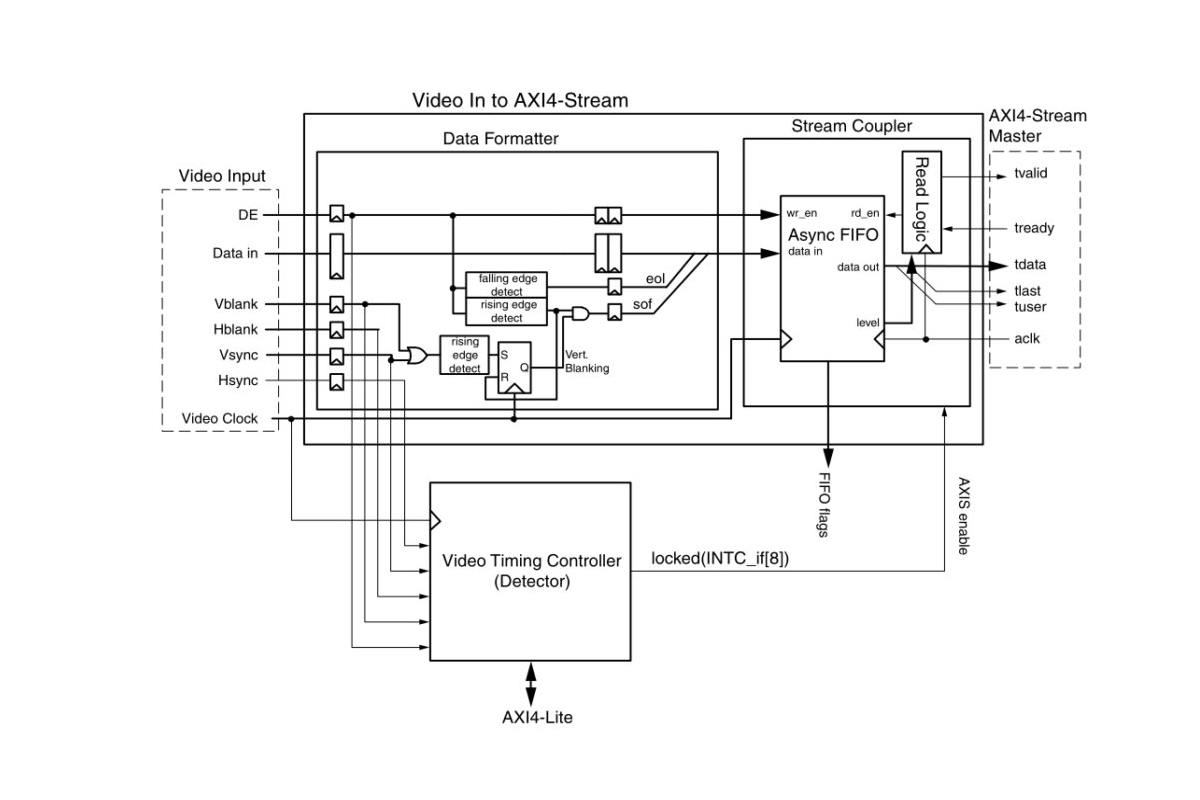
\includegraphics[width=14cm]{data4.png}
	\caption{Schemat połączenia w magistrali AXI4-Stream}
	\label{fig:Zynq3}
\end{figure}

\subsubsection{AXI SPI 1.02.a}
Moduł Xilinx AXI Serial Peripheral Interface (SPI) zapewnia komunikację z urządzeniami posiadającymi szeregowy interfejs urządzeń peryferyjnych [4]. W projekcie wykorzystywany jest do programowania przetwornika obrazu CMV 4000. Komunikacja odbywa się synchronicznie przy pomocy 4 standardowych sygnałów SPI:
\begin{itemize}
\item Master Out Slave In (MOSI)
\item Master In Slave Out (MISO)
\item Serial Clock (SCK)
\item Slave Select (SS)
\end{itemize}

Wewnętrzne rejestry modułu są programowane przez użytkownika poprzez interfejs AXI4 Lite. Ogólnie przyjętym standardem jest, że sygnał Slave Select jest aktywny poziomem niskim. W przypadku użytego sensora występuje sytuacja odwrotna – Slave Select jest aktywny poziomem wysokim, co wymagało stworzenia „przejściówki” w VHDL odwracającej wartość sygnału Slave Select.

\subsubsection{AXI Interconnect 1.06.a}
Moduł Xilinx AXI Interconnect łączy 1 lub więcej urządzeń nadrzędnych (master) AXI4 MM do 1 lub więcej urządzeń podrzędnych (slave) AXI4 MM. W projekcie moduły te zapewniają połączenie 1 do 1 pomiędzy czterema modułami AXI VDMA (master), a czterema łączami wysokiej przepustowości HP do kontrolera pamięci (slave) oraz pomiędzy interfejsem AXI4 Lite (master), a łączem ogólnego przeznaczenia GP (slave). W przypadku bieżącej wersji układu Zynq, moduł ten zapewnia także konwersję pomiędzy wersjami 3 i 4 protokołu AXI. Sprzętowo, od strony układu przetwarzania (PS) obsługiwana jest wersja 3 protokołu, natomiast moduły własności intelektualnej korzystają z wersji 4. Szczegółowy opis architektury moduł można znaleźć w \cite{5}.

\subsubsection{Cam – Control 1.00.a}
Cam Control jest bardzo prostym pod-modułem stworzonym w ramach projektu, służącym do sterowania Modułem Interfejsu Sensora. Składa się on z jednego 32 – bitowego rejestru, programowanego poprzez interfejs AXI4 Lite. Opis poszczególnych bitów rejestru sterującego: 0 – frame request 1 – reset modułu interfejsu sensora
Moduł Interfejsu Sensora Napisana w VHDL jednostka odpowiada za odbieranie i deserializację danych obrazowych z przetwornika oraz generację sygnałów zegarowych wewnętrznych oraz dla przetwornika. Jednostka została napisana na podstawie kodu VHDL firmy CMOSIS, służącego do obsługi sensora CMV4000 poprzez interfejs Camera Link. Kod firmy CMOSIS stworzony i przetestowany został na układzie Xilinx Virtex 4. Uruchomienie kodu na układzie Zynq i przystosowanie do potrzeb bieżącego projektu wymagało pewnych zmian.
Moduł interfejsu składa się z następujących plików źródłowych VHDL:
\begin{itemize}
\item  \textit{module\_1\_stub.vhd} Główny plik projektu, odpowiada za integrację interfejsu sensora z modułami IP oraz systemem przetwarzania Zynq. Zawiera opis połączeń modułów z sygnałami wyprowadzonymi na zewnątrz układu FPGA.

\item \textit{tsc\_mv1\_top.vhd} Nadrzędny plik modułu interfejsu sensora. Zawiera instancje wszystkich pozostałych podmodułów.

\item \textit{tsc\_mv1\_clocking.vhd} Plik modułu generacji zegara, zawiera instancję modułu zegarowego Xilinx Clocking Wizard v3.6.0. Odpowiada także za generację sygnałów resetu dla pozostałych podmodułów interfejsu sensora.

\item \textit{tsc\_mv1\_control.vhd} Plik zawiera implementację głównego automatu sterującego modułem interfejsu LVDS.

\item \textit{tsc\_mv1\_datapath.vhd} Plik zawiera instancję odbiornika LVDS.

\item \textit{tsc\_mv1\_rx.vhd} Główny plik odbiornika LVDS, zawiera instancje deserializerów LVDS dla poszczególnych kanałów sensora oraz automat sterujący trenowaniem interfejsu LVDS. Dla zaoszczędzenia zasobów logiki programowalnej, zaimplementowany został jeden kontroler trenujący, współdzielony przez wszystkie kanały LVDS. Trenowanie odbywa się sekwencyjnie, każdego kanału po kolei.

\item \textit{tsc\_mv1\_ser2par.vhd} Plik zawierający opis interfejsu odbiorczego LVDS. Uproszczony schemat przedstawiony jest na rysunku 6.

\item \textit{vid\_sig\_formatter.vhd} Plik zawierający opis modułu przesuwającego sygnały Data Valid i Frame Valid zgodnie z wymaganiami rdzenia Video in to AXI4 Stream.

\end{itemize}

\subsection{Interfejs odbiorczny LVDS}

\begin{figure}[H]
	\centering
	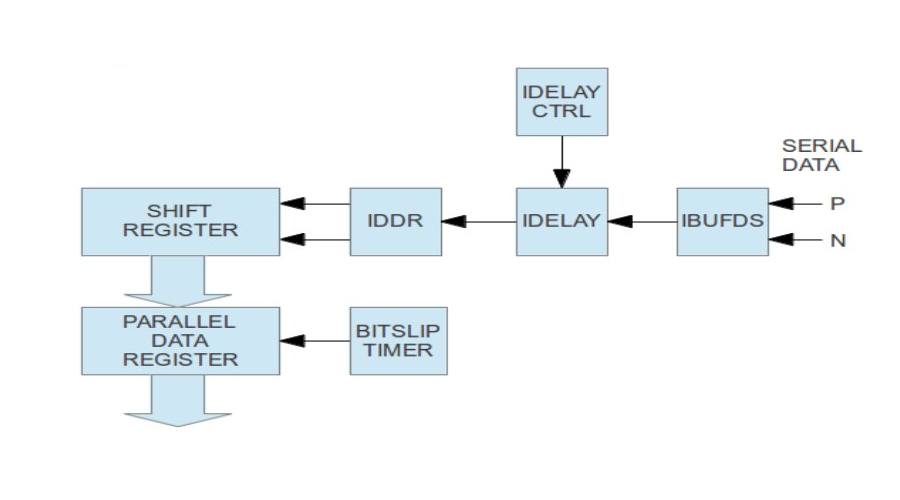
\includegraphics[width=16cm]{data5.png}
	\caption{Interfejs odbiorczy LVDS}
	\label{fig:Zynq5}
\end{figure}

Interfejs odbiorczy LVDS dla każdego kanału składa się z szeregu bloków funkcjonalnych. Pierwszym elementem jest IBUFDS – bufor odpowiedzialny za odbiór elektrycznego sygnału różnicowego i jego zamianę na na sygnał pojedynczy. Następnym elementem jest programowalny bufor opóźniający IDELAY, którego zadaniem jest wyrównanie opóźnień poszczególnych linii danych i zapewnienie optymalnego punktu próbkowania danej na zboczu zegarowym. W układach FPGA serii 7 (a więc także Zynq) bufor ten ma 32 stopniową skalę opóźnienia, a każdy krok opóźnia sygnał wejściowy o 78ps (Ref\_clk = 200MHz) [10], co razem daje prawie 2,5ns opóźnienia (1 okres zegara 400MHz). 

Blokiem współpracującym z IDELAY jest IDELAY CONTROL. Element ten na bieżąco kontroluje i kalibruje blok opóźniający uodporniając go na rozrzuty produkcyjne, zmiany temperatury oraz napięć zasilających (w pewnym zakresie) [11]. Po odpowiednim opóźnieniu sygnał trafia do bloku IDDR, który próbkuje sygnał na obu zboczach zegara danych i zamienia go na dwa sygnały wystawiane na pojedynczym zboczu. Następnie dane są kierowane do rejestru przesuwnego i rejestru wyjściowego, gdzie są zatrzaskiwane na sygnale wystawianym przez licznik modulo 10 (lub 12).

\subsection{Trenowanie interfejsu odbiorczego LVDS}
Ponieważ sensor nie generuje żadnych sygnałów ustalających początek kolejnego słowa w szeregowym strumieniu bitów, przed odbiorem danych interfejs musi zostać wytrenowany. Pierwszym krokiem algorytmu trenowania jest takie opóźnienie sygnałów z poszczególnych linii LVDS, aby znaleźć stabilny punkt próbkowania danych. Dokonuje tego automat sterujący, próbkujący wartość bitu słowa trenującego określoną ilość razy i porównując czy wartość bitu się zmieniła. Po każdej serii porównań, następuje opóźnienie sygnału o jeden krok i powtórzenie procedury od nowa. Po znalezieniu stabilnego regionu wartości bitu, wartość opóźnienia jest ustawiana tak, aby punkt próbkowania znalazł się w jego środku. 

Następnym krokiem jest ustalenie początku słowa danych. Odbywa się to poprzez porównywanie odebranych danych ze znanym wzorcem i przesuwanie danych w rejestrze przesuwnym, aż do momentu kiedy nastąpi zgodność ze wzorcem. Wartość przesunięcia zostaje zapamiętana i wykorzystana do odbioru właściwych danych. Dokładny opis algorytmu trenowania można znaleźć w \cite{12}.

\subsection{Główny automat sterujący}


Zaprojektowano prosty 8 – stanowy automat sterujący, którego zadaniem jest kierowanie pracą modułu interfejsu sensora. Po uruchomieniu układu FPGA, automat znajduje się w stanie INIT, z którego przechodzi do stanu RESET. W stanie RESET generowany jest sygnał resetu dla sensora, który podtrzymywany jest przez pewną ilość taktów zegara, odliczaną przy pomocy licznika. Następnie automat przechodzi do stanu IDLE w którym pozostaje, aż do otrzymania poziomu wysokiego sygnału CMD\_GRAB\_FRAME. 

Po otrzymaniu sygnału odczytu klatki następuje trenowanie interfejsu LVDS oraz oczekiwanie na pojawienie się sygnału FRAME\_VALID. Automat oczekuje sekwencji sygnału FRAME\_VALID o postaci 010, a po jej pojawieniu się powraca do stanu IDLE. Rozwiązanie takie pozwala na trenowanie interfejsu przed każdą klatką obrazu oraz testowanie stabilności sygnałów sterujących, ponieważ niewystąpienie którejś z wartości spodziewanej sekwencji spowoduje zawieszenie się automatu. W wersji produkcyjnej systemu, należy rozważyć inne scenariusze trenowania oraz sterowania interfejsem tak, aby układ był możliwie najbardziej odporny na zakłócenia. Projekt był testowany pod kątem stabilności – układ pracował przez kilka godzin z uruchomionym odczytem danych z sensora – w trakcie trwania testu nie doszło do zawieszenia automatu.

\begin{figure}[H]
	\centering
	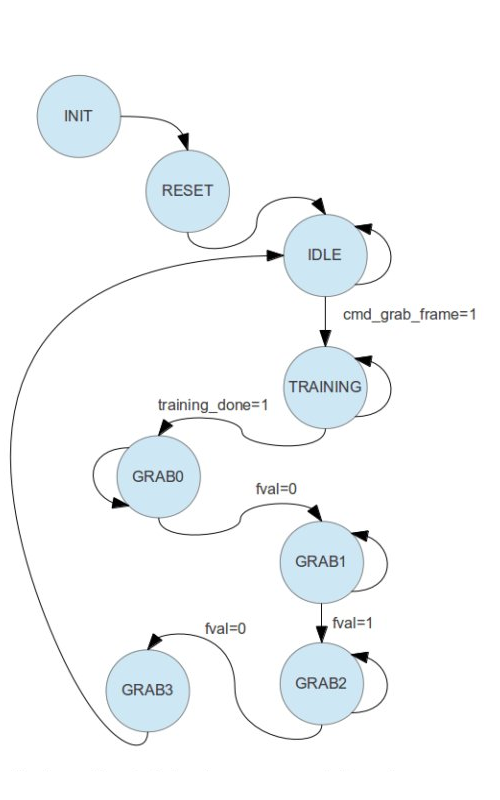
\includegraphics[width=8cm]{data6.png}
	\caption{Graf przejść głównego automatu sterującego}
	\label{fig:Zynq6}
\end{figure}

\subsection{Raport implementacji sprzętowej}
Projekt napisano i zaimplementowano przy użyciu oprogramowania Xilinx ISE Desing Suite w wersji 14.6. Projekt części sprzętowej został zrealizowany w programie PlanAhead oraz Xilinx Platform Studio. Implementacja zakończyła się poprawnie, zużyto maksymalnie połowę dostępnych zasobów. Widoczny 1 błąd nie dotyczy implementacji projektu, a jest wynikiem błędu w oprogramowaniu Xilinx. Szczegółowe raporty opisujące każdy etap syntezy oraz implementacji dostępne są w katalogu projektu.

\begin{figure}[H]
	\centering
	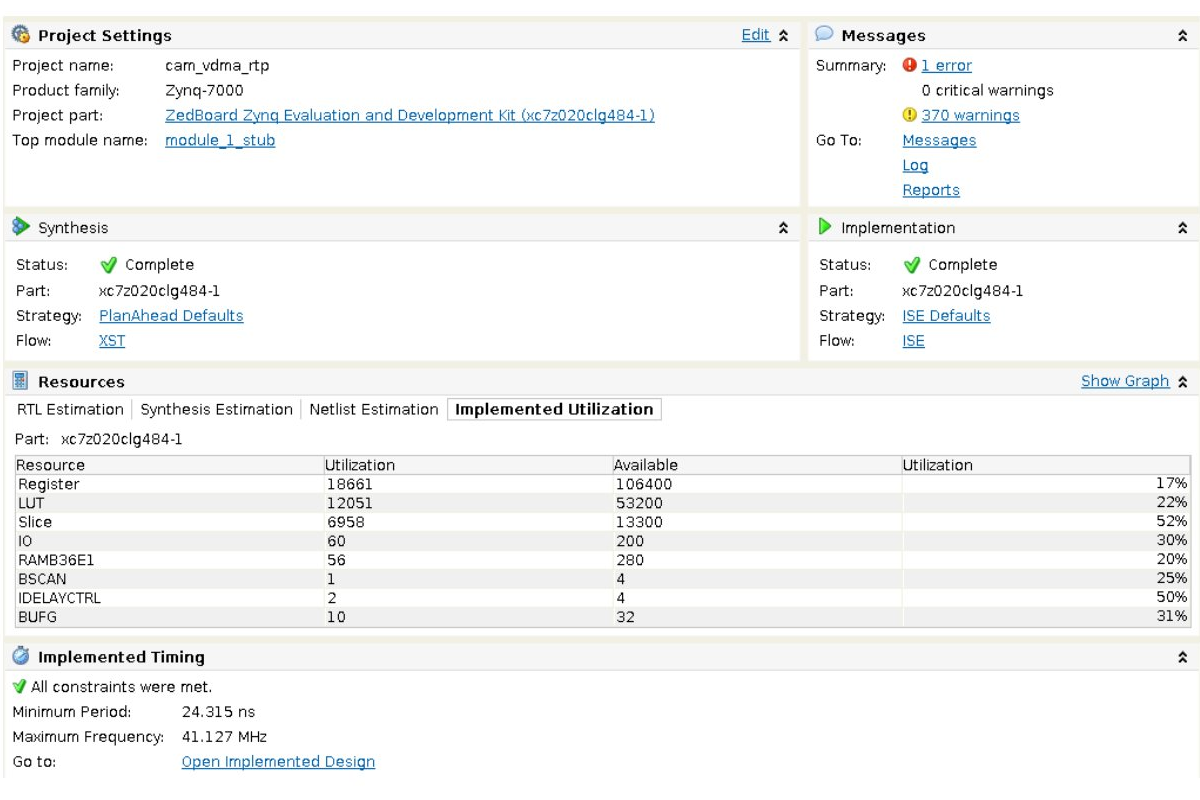
\includegraphics[width=16cm]{data7.png}
	\caption{Raport implementacji sprzętowej w programie PlanAhead}
	\label{fig:Zynq7}
\end{figure}

\section{Część programowa}
Część programową projektu napisano w języku C za pomocą środowiska programistycznego Xilinx SDK, będącego częścią ISE Design Suite.

\subsection{System operacyjny} 

Do sterowania sprzętem oraz komunikacji serwera z klientem wykorzystano prosty system operacyjny o otwartym kodzie źródłowym FreeRTOS [9] w wersji 7.0.2. Jest to system czasu rzeczywistego opracowany specjalnie dla systemów wbudowanych, charakteryzujący się prostotą, szybkością i bardzo małym wykorzystaniem zasobów. Wspiera wielozadaniowość, mechanizmy synchronizacji wątków oraz programowe liczniki czasu. Zapewnia podstawowe mechanizmy zarządzania pamięcią, zadania (wątki systemu) operują we wspólnej przestrzeni adresowej. FreeRTOS współpracuje z biblioteką lwIP, która zapewnia implementację stosu TCP/IP dla systemów wbudowanych, zaprojektowaną pod kątem minimalnego wykorzystania zasobów. W projekcie użyto bibliotekę lwIP w wersji 1.4.0. W projekcie wykorzystano 2 wersję algorytmu zarządzania stertą (heap\_2.c). Pozwala ona na rezerwowanie i zwalnianie bloków pamięci. Nie łączy ze sobą sąsiednich wolnych bloków, więc nie nadaje się do zastosowań gdzie tworzone i zwalniane są wątki o zróżnicowanym rozmiarze sterty. W projekcie taka sytuacje nie występuje, więc wersja 2 algorytmu jest wyborem optymalnym. Zrezygnowano z używania funkcji bibliotecznych dostarczanych przez Xilinx (malloc i free), ponieważ podczas testowania okazało się, że zachowują się niestabilnie – czasami podczas uruchamiania programu zwracają błąd niemożliwości przydziału pamięci, mimo że pamięć wcześniej nie była zajęta.

\subsection{Mapa przestrzeni adresowej}
Poniżej przedstawiono mapę adresów podstawowych komponentów projektu. Mapa nie wyczerpuje wszystkich elementów, pełną mapę można znaleźć w plikach projektu Xilinx Platform Studio.

\begin{figure}[H]
	\centering
	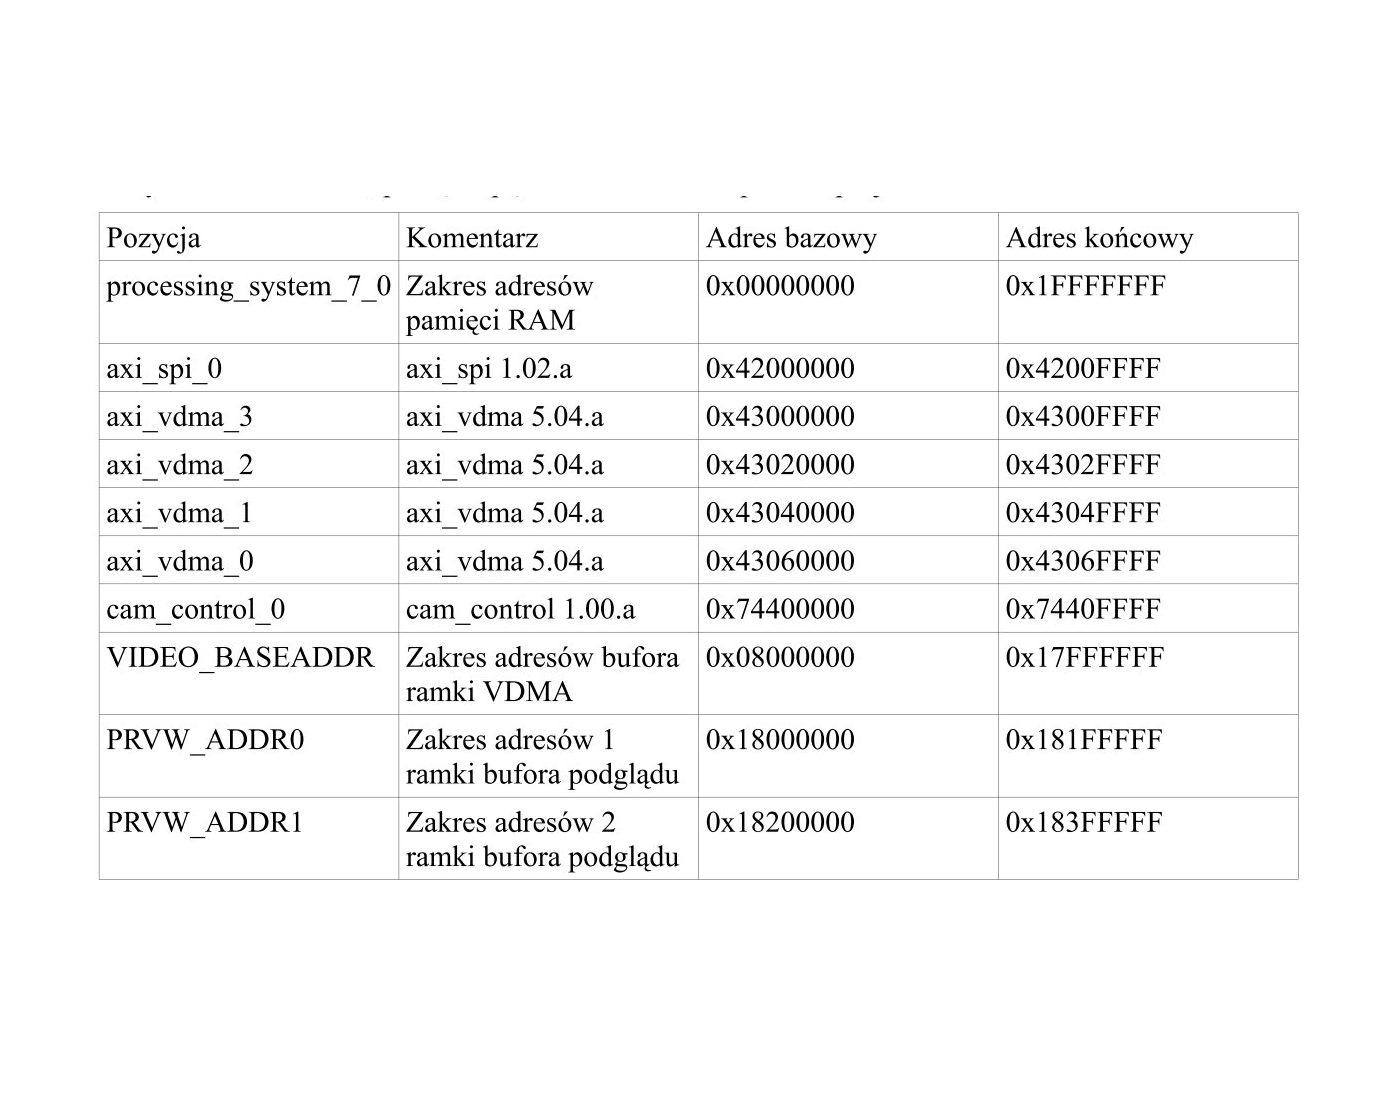
\includegraphics[width=16cm]{data8.png}
	\caption{Mapa adresów komponentów projektu}
	\label{fig:Zynq8}
\end{figure}

\subsection{Aplikacja serwera}

Oprogramowanie serwera stworzone na potrzeby projektu wykorzystuje obydwa rdzenie ARM Cortex A9 w trybie AMP (asymmetric multiprocessing). Tryb AMP pozwala na uruchomienie na każdym rdzeniu procesora oddzielnego systemu operacyjnego. Na rdzeniu CPU0 uruchamiany jest FreeRTOS, natomiast CPU1 pracuje bez żadnego systemu operacyjnego w tzw. trybie bare metal.
CPU0 odpowiada za:
\begin{itemize} 
\item Zarządzanie i programowanie układów peryferyjnych projektu w tym DMA • Komunikację z klientem przez Ethernet używając stosu lwIP 
\item pakietyzację RTP i strumieniowanie podglądu na żywo
\end{itemize}
CPU1 odpowiada za: 
\begin{itemize}
\item Obsługę przerwania od rdzenia IP AXI VIDEO DMA  
\item Konwersję oraz podwójne buforowanie danych obrazu do podglądu
\end{itemize}

Synchronizacja programów uruchomionych na poszczególnych rdzeniach procesora odbywa się za pomocą semaforów znajdujących się w pamięci OCM SRAM (przy wyłączonej pamięci podręcznej w obszarze jej adresów, zapewnia deterministyczny czas dostępu oraz mniejsze opóźnienie od pamięci DRAM). Obydwa rdzenie korzystają ze wspólnej przestrzeni adresowej, co wymusza ostrożne zarządzanie obszarami pamięci oraz adresowaniem.

\section{Realizacja programowa}



\section{Akwizycja danych z czujnika}

\section{System rejestracji parametrów lotu}

\section{Zapis danych}

\subsection{Interfejs SATA}



\chapter{Podsumowanie}





\begin{thebibliography}{9}
\bibitem{SPEC} Specyfikacja wymagań modułu odczytowgeo układu UFXC - Firmware
\bibitem{ZC706} Xilinx ZC706 Evaluation Board \url{http://www.xilinx.com/products/boards-and-kits/EK-Z7-ZC706-G.htm}
\bibitem{CMV4000} CMOSIS CMV4000 Sensor \url{http://www.cmosis.com/products/standard_products/cmv4000}
\bibitem{CIS} CIS 1910F Sensor
\bibitem{SPEC_PHOTO} \url{http://www.steadidrone.eu/uav-hexacopter-h6x-for-precise-agriculture/}
\bibitem{5}  LogiCORE IP AXI Interconnect v1.06.a, Xilinx, DS768 December 18, 2012
\bibitem{12} Application note for CMV2000 and CMV4000 , Interface Training , CMV2000-AN3-v1 , CMOSIS NV, 2009
\end{thebibliography}
\end{document}
